\begin{frame}{Introduction}
	\begin{columns}
		% Left Column: EEG Channels and Sleep Stages Table (Now on the Left Side)
		\column{0.50\textwidth}
		\textbf{SleepEDF Channels:}
		\begin{itemize}
			\item EEG Fpz-Cz
			\item EEG Pz-Oz
			\item EMG submental
			\item EOG horizontal
		\end{itemize}
		
		\vspace{10pt}
		
		\textbf{Sleep Stages and Frequency Ranges:}
		\begin{table}
			\centering
			\renewcommand{\arraystretch}{1.2}
			\begin{tabular}{|c|c|}
				\hline
				\textbf{Sleep Stage} & \textbf{Frequency (Hz)} \\
				\hline
				Wake (Beta) & 12-30 \\
				N1 (Light Sleep) & 4-8 \\
				N2 (Moderate Sleep) & 4-6 \\
				N3 (Deep Sleep) & 0.5-4 \\
				REM (Theta) & 4-6 \\
				\hline
			\end{tabular}
		\end{table}
		
		% Right Column: Figure (Now on the Right Side)
		\column{0.50\textwidth}
		\begin{figure}
			\centering
			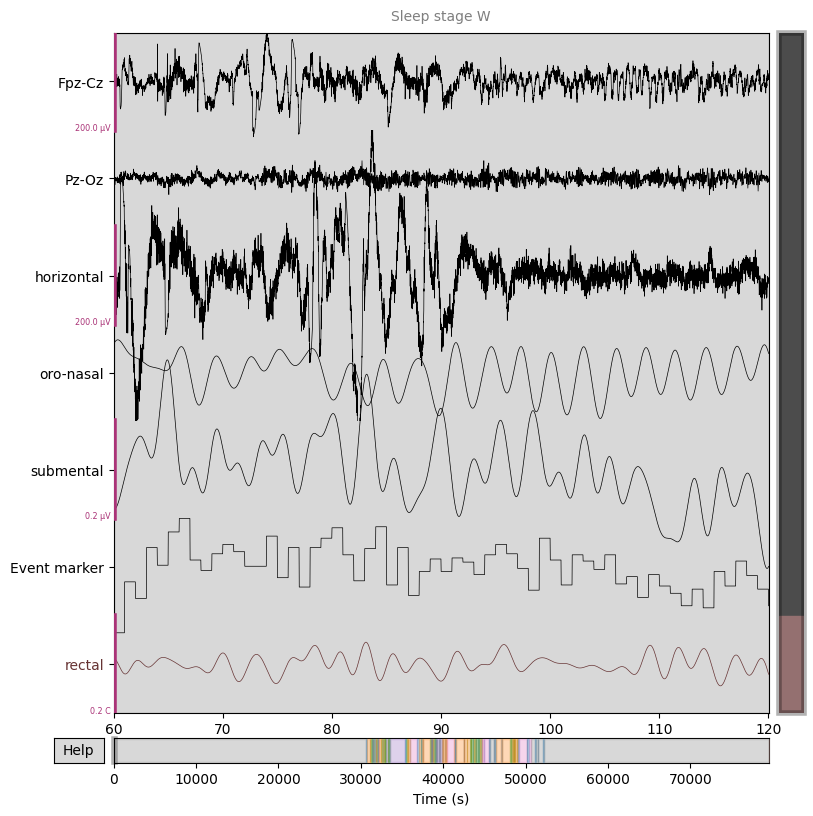
\includegraphics[width=\linewidth]{Sleep EDF Data Visulization.png} % Replace with your actual figure
			\caption{Sleep Stage Representation}
		\end{figure}
	\end{columns}
\end{frame}
